\documentclass[a4paper,11pt]{article}
\input{/home/tof/Documents/Cozy/latex-include/preambule_doc.tex}
\input{/home/tof/Documents/Cozy/latex-include/preambule_commun.tex}
\newcommand{\showprof}{show them}  % comment this line if you don't want to see todo environment
\setlength{\fboxrule}{0.8pt}
\fancyhead[L]{\fbox{\Large{\textbf{Archi 04}}}}
\fancyhead[C]{\textbf{Exercices listes chaînées}}
\newdate{madate}{10}{09}{2020}
%\fancyhead[R]{\displaydate{madate}} %\today
\fancyhead[R]{Terminale - NSI}
\fancyfoot[L]{\vspace{1mm}Christophe Viroulaud}
\AtEndDocument{\label{lastpage}}
\fancyfoot[C]{\textbf{Page \thepage/\pageref{lastpage}}}
\fancyfoot[R]{\includegraphics[width=2cm,align=t]{/home/tof/Documents/Cozy/latex-include/cc.png}}

\begin{document}
\begin{exo}
    \begin{framed}
        Essayer de réactiver sa mémoire avant de regarder le code vu en classe.
    \end{framed}
    \begin{enumerate}
        \item Écrire une classe \textbf{\texttt{Maillon}} avec deux attributs:
              \begin{itemize}
                  \item \textbf{\texttt{valeur: int}}
                  \item \textbf{\texttt{suivant: Maillon}}
              \end{itemize}
        \item Écrire une classe \textbf{\texttt{Liste}} avec un attribut \textbf{\texttt{tete: Maillon}} initialisé à \textbf{\texttt{None}}.
        \item Écrire la méthode \textbf{\texttt{ajouter(self, val: int) $\rightarrow$ None}} qui ajoute \textbf{\texttt{val}} à la liste.
        \item Instancier la liste et la remplir avec 10 entiers.
        \item Écrire la méthode \emph{impérative} \textbf{\texttt{dernier}} qui renvoie le dernier élément de la liste. La méthode renverra \textbf{\texttt{-1}} si la liste est vide.
        \item Proposer une version récursive de la méthode précédente.
        \item Sur papier, schématiser l'algorithme qui renverse l'ordre de la liste.
        \item Écrire alors la méthode \emph{impérative} \textbf{\texttt{renverser}}.
        \item Écrire la méthode \emph{impérative} \textbf{\texttt{dupliquer}} qui double chaque élément dans la liste. Par exemple: \textbf{\texttt{ 1 - 2 - 3}} devient \textbf{\texttt{1 - 1 - 2 - 2 - 3 - 3}}.
    \end{enumerate}
\end{exo}
\begin{exo}
    \begin{enumerate}
        \item Dans un nouveau fichier, importer les classes \textbf{\texttt{Liste, Maillon}} créées dans l'exercice précédant.
        \item Créer deux listes \textbf{\texttt{l1, l2}} et ajouter au moins trois entiers dans chaque liste.
        \item Écrire une fonction \textbf{\texttt{concatener(l1: Liste, l2: Liste) $\rightarrow$ Liste}} qui renverra une \textbf{\texttt{Liste}}, concaténation des deux passées en paramètre. Cette fonction contiendra une fonction interne \textbf{\texttt{concatener\_rec(tete1: Maillon, tete2: Maillon) $\rightarrow$ Maillon}} qui implémentera le principe de la figure \ref{concat}. On remarquera en particulier que cette fonction ne copie pas la \textbf{\texttt{Liste}} 2.
              \begin{center}
                  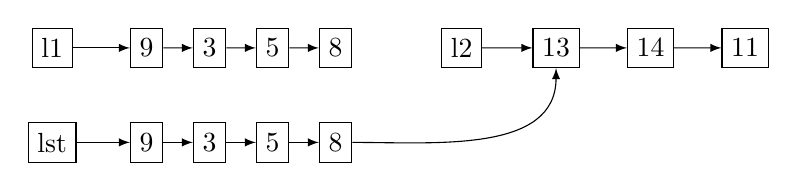
\begin{tikzpicture}[scale=0.4]
                      \node[draw,minimum height=0.5cm] (lst1) at (-13,2) {l1};
                      \node[draw,minimum height=0.5cm] (9) at (-10,2) {9};
                      \node[draw,minimum height=0.5cm] (3) at (-8,2) {3};
                      \node[draw,minimum height=0.5cm] (5) at (-6,2) {5};
                      \node[draw,minimum height=0.5cm] (8) at (-4,2) {8};

                      \draw[->,>=latex] (lst1) -- (9);
                      \draw[->,>=latex] (9) -- (3);
                      \draw[->,>=latex] (3) -- (5);
                      \draw[->,>=latex] (5) -- (8);

                      \node[draw,minimum height=0.5cm] (lst2) at (0,2) {l2};
                      \node[draw,minimum height=0.5cm] (13) at (3,2) {13};
                      \node[draw,minimum height=0.5cm] (14) at (6,2) {14};
                      \node[draw,minimum height=0.5cm] (11) at (9,2) {11};

                      \draw[->,>=latex] (lst2) -- (13);
                      \draw[->,>=latex] (13) -- (14);
                      \draw[->,>=latex] (14) -- (11);

                      \node[draw,minimum height=0.5cm] (lst) at (-13,-1) {lst};
                      \node[draw,minimum height=0.5cm] (92) at (-10,-1) {9};
                      \node[draw,minimum height=0.5cm] (32) at (-8,-1) {3};
                      \node[draw,minimum height=0.5cm] (52) at (-6,-1) {5};
                      \node[draw,minimum height=0.5cm] (82) at (-4,-1) {8};

                      \draw[->,>=latex] (lst) -- (92);
                      \draw[->,>=latex] (92) -- (32);
                      \draw[->,>=latex] (32) -- (52);
                      \draw[->,>=latex] (52) -- (82);
                      \draw[->,>=latex] (82) to[out=0,in=270] (13);

                  \end{tikzpicture}
                  \captionof{figure}{Fonctionnement de \textbf{concatener\_rec}}
                  \label{concat}
              \end{center}
        \item Quel problème peut-on prévoir lors de la modification d'un élément de la \textbf{\texttt{Liste}}?
        \item Estimer la complexité de la concaténation.
    \end{enumerate}
\end{exo}
\begin{exo}
    On décide de créer une liste chaînée à l'aide de tuples.
    \begin{center}
        \begin{lstlisting}[language=Python  , xleftmargin=2em, xrightmargin=2em]
lst = ("a", ("b", ("c", ("d", ()))))
\end{lstlisting}
        \captionof{code}{"a" est la tête de la liste}
        \label{CODE}
    \end{center}
    \begin{enumerate}
        \item Écrire la fonction \textbf{\texttt{longueur(lst: tuple) $\rightarrow$ int}} qui renvoie la taille de la liste.
        \item Écrire la fonction \textbf{\texttt{afficher(lst: tuple) $\rightarrow$ str}} qui renvoie une chaîne de caractère de la forme
              \begin{lstlisting}[language=Python  , xleftmargin=2em, xrightmargin=2em]
a - b - c - d - fin
\end{lstlisting}
    \end{enumerate}
\end{exo}
\end{document}